\documentclass[xcolor=dvipsnames]{beamer} % dvipsnames gives more built-in colors
\mode<presentation>

\usetheme{Boadilla}

\definecolor{GWdarkblue}{HTML}{033C5A}

\usecolortheme[named=GWdarkblue]{structure}

% Sets the font
\usepackage[defaultfam,tabular,lining]{montserrat}
\setbeamerfont{title}{shape=\scshape}
\setbeamerfont{frametitle}{shape=\scshape}
%Remove "Figure" from captions
\setbeamertemplate{caption}{\raggedright\insertcaption\par}

\usepackage{graphicx}
\usepackage{tabularx}
\usepackage{hyperref}

\usepackage{soul}
\makeatletter
\let\HL\hl
\renewcommand\hl{%
  \let\set@color\beamerorig@set@color
  \let\reset@color\beamerorig@reset@color
  \HL}
\makeatother

\title[Hypothesis Testing]{Hypothesis Testing}
\author[SMPA 2152]{Data Analysis for Journalism and Political Communication (Spring 2025)}
\date{Prof. Bell}

\begin{document}

%%%%%%%%%%%%%%%%%%%%%%%%%%%%%%%%%%%%%%%%%%%%%%%%%%%%%%%%%%%%%%%%%%
\frame{
\titlepage
}

%%%%%%%%%%%%%%%%%%%%%%%%%%%%%%%%%%%%%%%%%%%%%%%%%%%%%%%%%%%%%%%%%%
\frame{\frametitle{Writing Hypotheses}

Every hypothesis has \underline{two} opposing versions, both of which are critically important:

\begin{enumerate}
    \item The null hypothesis ($H_0$), also called ``H-naught''
    \item The alternative hypothesis ($H_A$ or $H_1$)
\end{enumerate}
~\\
\begin{itemize}[<+(1)->]
    \item $H_0$ is the hypothesis of ``not''. For example:
    \begin{itemize}
        \item<.-> $H_0$: Voters who decided in the last month were \textbf{not} more likely to support Donald Trump than Kamala Harris.
    \end{itemize}
    \item $H_A$ is the hypothesis of \textbf{difference}. For example:
    \begin{itemize}
        \item<.-> $H_A$: Voters who decided in the last month were more likely to support Donald Trump than Kamala Harris.
    \end{itemize}
\end{itemize}
}

%%%%%%%%%%%%%%%%%%%%%%%%%%%%%%%%%%%%%%%%%%%%%%%%%%%%%%%%%%%%%%%%%%
\frame{\frametitle{Let's Practice}

Identify whether each of these hypotheses is $H_0$ or $H_A$, and provide it's opposite:

\begin{enumerate}
    \item \only<2->{$H_0$: }Global temperatures are not different today than they were 50 years ago.
        \only<2->{~\\\hl{$H_A$: Global temperatures are higher today than they were 50 years ago.}}
    \item \only<3->{$H_A$: }Regular viewers of 24-hour news channels are more partisan than non-viewers.
        \only<3->{~\\\hl{$H_0$: Regular viewers of 24-hour news channels are not more partisan as non-viewers.}}
    \item \only<4->{$H_A$: }The number of soldiers from a voter's area who are killed in Iraq is correlated with votes for John Kerry in the 2004 presidential election.
        \only<4->{~\\\hl{$H_0$: The number of soldiers from a voter's area who are killed in Iraq is not correlated with votes for John Kerry in the 2004 presidential election.}}
\end{enumerate}
}

%%%%%%%%%%%%%%%%%%%%%%%%%%%%%%%%%%%%%%%%%%%%%%%%%%%%%%%%%%%%%%%%%%
\frame{\frametitle{Intuition of Hypothesis Testing}

\begin{itemize}[<+->]
    \item Our goal is to show that $H_0$ is very unlikely to be true.
    \item Why? Because we want to avoid Type I error (false positives where we incorrectly claim that $H_A$ is true).
    \begin{itemize}
        \item This is why we say that the criminal justice system has a presumption of innocence:
        ~\\
        ~\\ $H_0$: The person is not guilty.
        ~\\ $H_A$: The person is guilty.
    \end{itemize}
    \item To do this, we assume a world in which $H_0$ is true, and place the burden on us (the prosecution) to show that this assumption is likely wrong.
    \item \textbf{We can never prove or disprove $H_0$}. We can only generate enough evidence to \textit{reject} $H_0$ or \textit{fail to reject} $H_0$.
\end{itemize}
}

%%%%%%%%%%%%%%%%%%%%%%%%%%%%%%%%%%%%%%%%%%%%%%%%%%%%%%%%%%%%%%%%%%
\frame{
In-class example
}

%%%%%%%%%%%%%%%%%%%%%%%%%%%%%%%%%%%%%%%%%%%%%%%%%%%%%%%%%%%%%%%%%%
\frame{\frametitle{Types of Hypothesis Tests}

\only<1>{
\begin{block}{One-sample t-test}
A difference-of-means test comparing an estimate of the mean to a specific alternative mean (often 0)
\end{block}
~\\
~\\
\begin{block}{Two-sample t-test}
A difference-of-means test comparing estimates of the mean of two samples
\end{block}
}

\only<2>{
\begin{block}{One-tailed t-test}
A difference-of-means test of whether an estimate of the mean is greater or less than an alternative (mean or sample)
\end{block}
~\\
~\\
\begin{block}{Two-tailed t-test}
A difference-of-means test of whether an estimate of the mean is different than an alternative (mean or sample)
\end{block}
{\footnotesize $^*$Most researchers use two-tailed tests even when they hypothesize a directional difference (greater or lesser) because a two-tailed test is more conservative and less likely to result in Type 1 error.}
}
}

%%%%%%%%%%%%%%%%%%%%%%%%%%%%%%%%%%%%%%%%%%%%%%%%%%%%%%%%%%%%%%%%%%
\frame{
Return to the in-class example
}

%%%%%%%%%%%%%%%%%%%%%%%%%%%%%%%%%%%%%%%%%%%%%%%%%%%%%%%%%%%%%%%%%%
\frame{\frametitle{Real-world Example}

\footnotesize
``Working Twice as Hard to Get Half as Far: Race, Work Ethic, and America’s Deserving Poor''\\
Christopher D. DeSante, \textit{Am. Journal of Political Science} vol. 57 iss. 2 (2013)
~\\
~\\
\centering
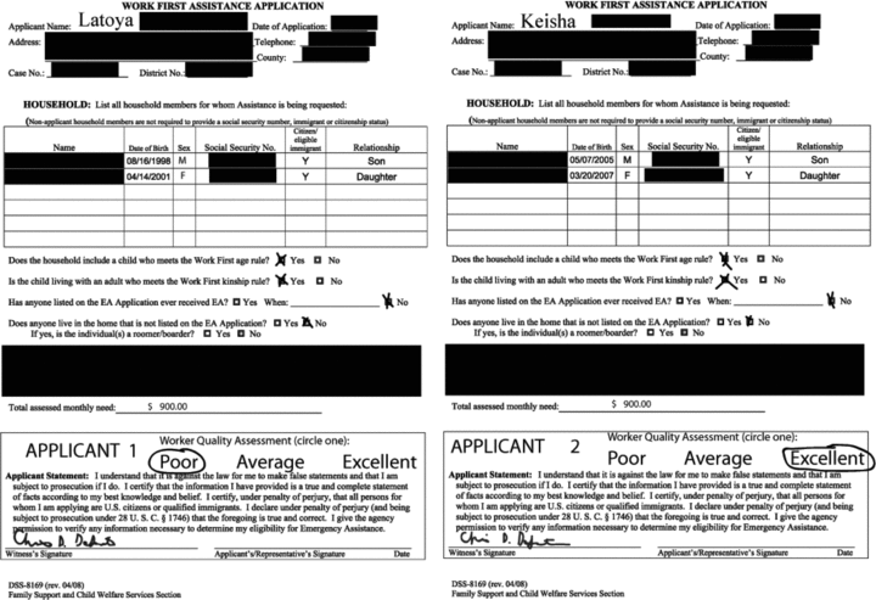
\includegraphics[height = .8\textheight]{desante_treatment.png}
}

\end{document}
